%% LyX 2.1.1 created this file.  For more info, see http://www.lyx.org/.
%% Do not edit unless you really know what you are doing.
\documentclass[12pt]{article}\usepackage[]{graphicx}\usepackage[]{color}
%% maxwidth is the original width if it is less than linewidth
%% otherwise use linewidth (to make sure the graphics do not exceed the margin)
\makeatletter
\def\maxwidth{ %
  \ifdim\Gin@nat@width>\linewidth
    \linewidth
  \else
    \Gin@nat@width
  \fi
}
\makeatother

\definecolor{fgcolor}{rgb}{0.345, 0.345, 0.345}
\newcommand{\hlnum}[1]{\textcolor[rgb]{0.686,0.059,0.569}{#1}}%
\newcommand{\hlstr}[1]{\textcolor[rgb]{0.192,0.494,0.8}{#1}}%
\newcommand{\hlcom}[1]{\textcolor[rgb]{0.678,0.584,0.686}{\textit{#1}}}%
\newcommand{\hlopt}[1]{\textcolor[rgb]{0,0,0}{#1}}%
\newcommand{\hlstd}[1]{\textcolor[rgb]{0.345,0.345,0.345}{#1}}%
\newcommand{\hlkwa}[1]{\textcolor[rgb]{0.161,0.373,0.58}{\textbf{#1}}}%
\newcommand{\hlkwb}[1]{\textcolor[rgb]{0.69,0.353,0.396}{#1}}%
\newcommand{\hlkwc}[1]{\textcolor[rgb]{0.333,0.667,0.333}{#1}}%
\newcommand{\hlkwd}[1]{\textcolor[rgb]{0.737,0.353,0.396}{\textbf{#1}}}%

\usepackage{framed}
\makeatletter
\newenvironment{kframe}{%
 \def\at@end@of@kframe{}%
 \ifinner\ifhmode%
  \def\at@end@of@kframe{\end{minipage}}%
  \begin{minipage}{\columnwidth}%
 \fi\fi%
 \def\FrameCommand##1{\hskip\@totalleftmargin \hskip-\fboxsep
 \colorbox{shadecolor}{##1}\hskip-\fboxsep
     % There is no \\@totalrightmargin, so:
     \hskip-\linewidth \hskip-\@totalleftmargin \hskip\columnwidth}%
 \MakeFramed {\advance\hsize-\width
   \@totalleftmargin\z@ \linewidth\hsize
   \@setminipage}}%
 {\par\unskip\endMakeFramed%
 \at@end@of@kframe}
\makeatother

\definecolor{shadecolor}{rgb}{.97, .97, .97}
\definecolor{messagecolor}{rgb}{0, 0, 0}
\definecolor{warningcolor}{rgb}{1, 0, 1}
\definecolor{errorcolor}{rgb}{1, 0, 0}
\newenvironment{knitrout}{}{} % an empty environment to be redefined in TeX

\usepackage{alltt}
\usepackage{mathptmx}
\usepackage[T1]{fontenc}
\usepackage[letterpaper]{geometry}
\geometry{verbose,tmargin=3.54cm,bmargin=2.54cm,lmargin=2.54cm,rmargin=2.54cm,headheight=1cm,headsep=2cm,footskip=0.5cm}
\usepackage{fancyhdr}
\pagestyle{fancy}
\setcounter{secnumdepth}{2}
\setcounter{tocdepth}{2}
\setlength{\parskip}{\medskipamount}
\setlength{\parindent}{0pt}
\usepackage{color}

\makeatletter

%%%%%%%%%%%%%%%%%%%%%%%%%%%%%% LyX specific LaTeX commands.
%% Because html converters don't know tabularnewline
\providecommand{\tabularnewline}{\\}

%%%%%%%%%%%%%%%%%%%%%%%%%%%%%% User specified LaTeX commands.
\input colordvi
\usepackage{color}
\fancyhead{}
\fancyfoot[CE,CO]{}
\newtoks{\addressee} \global\addressee={}
\newdimen\longindent \longindent=3.5truein
\fancyhead[L]{Memo to: \the\addressee \\ \datetoday \\ Page \thepage \hfill}
\renewcommand{\headrulewidth}{0.0pt}
\newenvironment{lyxlist}[1]
{\begin{list}{}
{\settowidth{\labelwidth}{#1}
\setlength{\leftmargin}{\labelwidth}
\addtolength{\leftmargin}{\labelsep}
\renewcommand{\makelabel}[1]{##1\hfil}}}
{\end{list}}
\newcommand{\datetoday}{\number\day\space
     \ifcase\month\or January\or February\or March\or April\or May\or
     June\or July\or August\or September\or October\or November\or
     December\fi
     \space\number\year}
\newcommand{\EOLmemo}{\null \vskip-1.5truein
{\raggedright \textsf{\textsc{\large \textcolor{blue}{Earth Observing Laboratory}}}}\par
{\raggedright \textsf{\textsl{\textcolor{blue}{Memorandum:}}}} \par \vskip6pt
{\color{blue}{\hrule}}\par
\vskip0.3truein \leftline{\hskip \longindent \datetoday} \vskip0.2truein
\thispagestyle{empty}}
\newcommand{\attachm}[1]{\begin{lyxlist}{Attachments:00}
\item [Attachments:] {#1}
\end{lyxlist}}
\newcommand{\cc}[1]{\begin{lyxlist}{Attachments:00}
\item [cc:] {#1}
\end{lyxlist}}
\newcommand{\attach}[1]{\begin{lyxlist}{Attachments:00}
\item [Attachment:] {#1}
\end{lyxlist}}
%usage: \encl{A\\B\\C} or \cc{ma,e1\\name2\\name3}

\makeatother
\IfFileExists{upquote.sty}{\usepackage{upquote}}{}
\begin{document}
\EOLmemo 

\global\addressee={RSessions file}  % >>change "File" to the "To:" name desired

\begin{tabular}{ll}
\textsf{\textsc{\textcolor{blue}{To:}}} & \the\addressee\tabularnewline
\textsf{\textsc{\textcolor{blue}{From:}}} & Al Cooper\tabularnewline
\textsf{\textsc{\textcolor{blue}{Subject:}}} & Using data.frame objects\tabularnewline
\end{tabular}

\bigskip


\section*{What is a data.frame?}

A data.frame resembles a matrix or a spreadsheet. For example, it
may consists of columns each representing a variable and rows that
are the time sequence of observations of that variable. Applied to
RAF data files, it may have a structure like this:

\noindent \begin{center}
\begin{tabular}{|c|c|c|c|c|c|}
\hline 
Time & ATX & PSXC & WDC & WSC & ...\tabularnewline
\hline 
\hline 
15:00:00 & -25.1 & 410.8 & 275.4 & 25.4 & ...\tabularnewline
\hline 
15:00:01 & -25.1 & 410.9 & 275.2 & 25.6 & ...\tabularnewline
\hline 
15:00:02 & -25.2 & 411.1 & 275.4 & 25.5 & ...\tabularnewline
\hline 
15:00:03 & -25.1 & 411.1 & 275.1 & 25.7 & ...\tabularnewline
\hline 
15:00:04 & -25.0 & 411.2 & 275.3 & 25.3 & ...\tabularnewline
\hline 
... & ... & ... & ... & ... & ...\tabularnewline
\hline 
\end{tabular}
\par\end{center}

All columns must be of the same length, but they may contain different
types of variables (Time, character, numeric, logical). Like a spreadsheet,
the columns can be assigned names like the header in this table. Rows
can also be assigned names, but in the absence of special assignment
they will default to the character names '1', '2', '3', '4', ...

Let's get an example. Here is a segment of R code that loads a few
selected variables from a netCDF file to a data.frame:

\begin{knitrout}
\definecolor{shadecolor}{rgb}{0.969, 0.969, 0.969}\color{fgcolor}\begin{kframe}
\begin{alltt}
\hlkwd{require}\hlstd{(Ranadu,} \hlkwc{quietly} \hlstd{=} \hlnum{TRUE}\hlstd{,} \hlkwc{warn.conflicts}\hlstd{=}\hlnum{FALSE}\hlstd{)} \hlcom{# my package of routines }
\end{alltt}


{\ttfamily\noindent\itshape\color{messagecolor}{\#\# Loading required package: RJSONIO\\\#\# \\\#\# Attaching package: 'signal'\\\#\# \\\#\# The following objects are masked from 'package:stats':\\\#\# \\\#\#\ \ \ \  filter, poly}}\begin{alltt}
\hlstd{Directory} \hlkwb{<-} \hlkwd{DataDirectory} \hlstd{()}    \hlcom{# for portability; sets the local data directory}
\hlstd{Flight} \hlkwb{<-} \hlstr{"rf08"}                 \hlcom{# select a flight}
\hlstd{Project} \hlkwb{=} \hlstr{"CONTRAST"}             \hlcom{# select a project}
\hlstd{fname} \hlkwb{=} \hlkwd{sprintf}\hlstd{(}\hlstr{"%s%s/%s%s.nc"}\hlstd{, Directory,Project,Project,Flight)}
\hlcom{# XXX set variables needed, here a standard list plus GGVSPDB}
\hlstd{Data} \hlkwb{<-} \hlkwd{getNetCDF} \hlstd{(fname,} \hlkwd{standardVariables}\hlstd{(}\hlkwd{c}\hlstd{(}\hlstr{"GGVSPDB"}\hlstd{)),} \hlnum{60000}\hlstd{,} \hlnum{60010}\hlstd{)}
\hlstd{saveDataFile} \hlkwb{<-} \hlstr{'RSessionsDataFrame.Rdata.gz'}
\hlkwd{save} \hlstd{(Data,} \hlkwc{file} \hlstd{= saveDataFile,} \hlkwc{compress}\hlstd{=}\hlstr{'gzip'}\hlstd{)}
\hlstd{N} \hlkwb{<-} \hlkwd{names}\hlstd{(Data)}
\end{alltt}
\end{kframe}
\end{knitrout}

The resulting names are Time, ATX, DPXC, EWX, GGALT, LATC, LONC, MACHX, MR, PALT, PSXC, QCXC, TASX, WDC, WSC, WIC, GGVSPDB. The data.frame 'Data' looks like
this:

\begin{knitrout}
\definecolor{shadecolor}{rgb}{0.969, 0.969, 0.969}\color{fgcolor}\begin{kframe}
\begin{verbatim}
##                   Time    ATX     DPXC   EWX GGALT  LATC  LONC  MACHX
## 1  2014-02-01 06:00:00  9.664 -1.74589 5.380  3271 14.14 154.3 0.5517
## 2  2014-02-01 06:00:01  9.600 -0.58043 5.860  3258 14.14 154.3 0.5523
## 3  2014-02-01 06:00:02  9.608 -0.10240 6.067  3245 14.14 154.3 0.5524
## 4  2014-02-01 06:00:03  9.649  0.04999 6.135  3231 14.14 154.3 0.5525
## 5  2014-02-01 06:00:04  9.745  0.18771 6.197  3218 14.14 154.3 0.5521
## 6  2014-02-01 06:00:05  9.832  0.30350 6.249  3205 14.14 154.3 0.5522
## 7  2014-02-01 06:00:06  9.898  0.65490 6.410  3191 14.14 154.3 0.5525
## 8  2014-02-01 06:00:07  9.972  0.56748 6.369  3178 14.15 154.3 0.5528
## 9  2014-02-01 06:00:08 10.021  0.50978 6.342  3164 14.15 154.3 0.5536
## 10 2014-02-01 06:00:09 10.103  0.45882 6.319  3151 14.15 154.3 0.5537
## 11 2014-02-01 06:00:10 10.179  0.53403 6.354  3137 14.15 154.3 0.5538
##       MR PALT  PSXC  QCXC  TASX   WDC   WSC     WIC GGVSPDB
## 1  4.866 3091 693.0 159.2 185.9 59.76 10.64 -0.2153  -13.53
## 2  5.295 3078 694.2 159.9 186.1 57.36 10.54 -0.2423  -13.41
## 3  5.475 3064 695.4 160.2 186.2 56.32 10.52 -0.3595  -13.37
## 4  5.528 3052 696.4 160.5 186.2 55.32 10.58 -0.3402  -13.30
## 5  5.575 3039 697.6 160.5 186.1 54.89 10.55 -0.3907  -13.34
## 6  5.613 3027 698.7 160.8 186.2 53.42 10.54 -0.4517  -13.40
## 7  5.750 3015 699.8 161.3 186.3 51.61 10.53 -0.4760  -13.46
## 8  5.704 3001 701.0 161.7 186.4 49.83 10.57 -0.5229  -13.49
## 9  5.671 2989 702.0 162.5 186.7 47.27 10.72 -0.5907  -13.52
## 10 5.640 2976 703.2 162.9 186.8 45.96 10.79 -0.6423  -13.52
## 11 5.662 2963 704.4 163.2 186.8 44.47 10.80 -0.6980  -13.58
\end{verbatim}
\end{kframe}
\end{knitrout}


\section*{Working with data.frames}


\subsection*{Addressing elements of a data.frame}

You can address particular elements using syntax like the following:

\begin{knitrout}
\definecolor{shadecolor}{rgb}{0.969, 0.969, 0.969}\color{fgcolor}\begin{kframe}
\begin{alltt}
\hlstd{Data}\hlopt{$}\hlstd{ATX[}\hlnum{5}\hlstd{]}
\end{alltt}
\begin{verbatim}
## [1] 9.745
\end{verbatim}
\begin{alltt}
\hlstd{Data[}\hlnum{5}\hlstd{,} \hlnum{2}\hlstd{]}           \hlcom{# note the [row,column] syntax}
\end{alltt}
\begin{verbatim}
## [1] 9.745
\end{verbatim}
\begin{alltt}
\hlstd{Data[}\hlnum{5}\hlstd{, ]}
\end{alltt}
\begin{verbatim}
##                  Time   ATX   DPXC   EWX GGALT  LATC  LONC  MACHX    MR
## 5 2014-02-01 06:00:04 9.745 0.1877 6.197  3218 14.14 154.3 0.5521 5.575
##   PALT  PSXC  QCXC  TASX   WDC   WSC     WIC GGVSPDB
## 5 3039 697.6 160.5 186.1 54.89 10.55 -0.3907  -13.34
\end{verbatim}
\begin{alltt}
\hlstd{Data[}\hlnum{5}\hlstd{,} \hlstr{"ATX"}\hlstd{]}
\end{alltt}
\begin{verbatim}
## [1] 9.745
\end{verbatim}
\begin{alltt}
\hlstd{Data}\hlopt{$}\hlstd{ATX}
\end{alltt}
\begin{verbatim}
##  [1]  9.664  9.600  9.608  9.649  9.745  9.832  9.898  9.972 10.021 10.103
## [11] 10.179
\end{verbatim}
\begin{alltt}
\hlstd{Data}\hlopt{$}\hlstd{ATX[}\hlkwd{getIndex}\hlstd{(Data}\hlopt{$}\hlstd{Time,} \hlnum{60004}\hlstd{)]}
\end{alltt}
\begin{verbatim}
## [1] 9.745
\end{verbatim}
\begin{alltt}
\hlstd{Data}\hlopt{$}\hlstd{ATX[Data}\hlopt{$}\hlstd{Time} \hlopt{==} \hlkwd{as.POSIXct}\hlstd{(}\hlstr{"2014-02-01 6:00:04"}\hlstd{,} \hlkwc{tz}\hlstd{=}\hlstr{'UTC'}\hlstd{)]}
\end{alltt}
\begin{verbatim}
## [1] 9.745
\end{verbatim}
\end{kframe}
\end{knitrout}


\subsection*{Creating subsets of a data.frame}

New data.frames that contain subsets of original data.frames can be
created using logical vectors. For example:

\begin{knitrout}
\definecolor{shadecolor}{rgb}{0.969, 0.969, 0.969}\color{fgcolor}\begin{kframe}
\begin{alltt}
\hlstd{Data[Data}\hlopt{$}\hlstd{TASX} \hlopt{>} \hlnum{186.2}\hlstd{, ]}
\end{alltt}
\begin{verbatim}
##                   Time    ATX    DPXC   EWX GGALT  LATC  LONC  MACHX    MR
## 4  2014-02-01 06:00:03  9.649 0.04999 6.135  3231 14.14 154.3 0.5525 5.528
## 7  2014-02-01 06:00:06  9.898 0.65490 6.410  3191 14.14 154.3 0.5525 5.750
## 8  2014-02-01 06:00:07  9.972 0.56748 6.369  3178 14.15 154.3 0.5528 5.704
## 9  2014-02-01 06:00:08 10.021 0.50978 6.342  3164 14.15 154.3 0.5536 5.671
## 10 2014-02-01 06:00:09 10.103 0.45882 6.319  3151 14.15 154.3 0.5537 5.640
## 11 2014-02-01 06:00:10 10.179 0.53403 6.354  3137 14.15 154.3 0.5538 5.662
##    PALT  PSXC  QCXC  TASX   WDC   WSC     WIC GGVSPDB
## 4  3052 696.4 160.5 186.2 55.32 10.58 -0.3402  -13.30
## 7  3015 699.8 161.3 186.3 51.61 10.53 -0.4760  -13.46
## 8  3001 701.0 161.7 186.4 49.83 10.57 -0.5229  -13.49
## 9  2989 702.0 162.5 186.7 47.27 10.72 -0.5907  -13.52
## 10 2976 703.2 162.9 186.8 45.96 10.79 -0.6423  -13.52
## 11 2963 704.4 163.2 186.8 44.47 10.80 -0.6980  -13.58
\end{verbatim}
\begin{alltt}
\hlstd{Data[}\hlkwd{setRange}\hlstd{(Data}\hlopt{$}\hlstd{Time,} \hlnum{60005}\hlstd{,} \hlnum{60008}\hlstd{), ]}
\end{alltt}
\begin{verbatim}
##                  Time    ATX   DPXC   EWX GGALT  LATC  LONC  MACHX    MR
## 6 2014-02-01 06:00:05  9.832 0.3035 6.249  3205 14.14 154.3 0.5522 5.613
## 7 2014-02-01 06:00:06  9.898 0.6549 6.410  3191 14.14 154.3 0.5525 5.750
## 8 2014-02-01 06:00:07  9.972 0.5675 6.369  3178 14.15 154.3 0.5528 5.704
## 9 2014-02-01 06:00:08 10.021 0.5098 6.342  3164 14.15 154.3 0.5536 5.671
##   PALT  PSXC  QCXC  TASX   WDC   WSC     WIC GGVSPDB
## 6 3027 698.7 160.8 186.2 53.42 10.54 -0.4517  -13.40
## 7 3015 699.8 161.3 186.3 51.61 10.53 -0.4760  -13.46
## 8 3001 701.0 161.7 186.4 49.83 10.57 -0.5229  -13.49
## 9 2989 702.0 162.5 186.7 47.27 10.72 -0.5907  -13.52
\end{verbatim}
\end{kframe}
\end{knitrout}

Another useful subset is that omitting all missing-variable rows from
the data.frame:

\begin{knitrout}
\definecolor{shadecolor}{rgb}{0.969, 0.969, 0.969}\color{fgcolor}\begin{kframe}
\begin{alltt}
\hlkwd{na.omit}\hlstd{(Data)}
\end{alltt}
\begin{verbatim}
##                   Time    ATX     DPXC   EWX GGALT  LATC  LONC  MACHX
## 1  2014-02-01 06:00:00  9.664 -1.74589 5.380  3271 14.14 154.3 0.5517
## 2  2014-02-01 06:00:01  9.600 -0.58043 5.860  3258 14.14 154.3 0.5523
## 3  2014-02-01 06:00:02  9.608 -0.10240 6.067  3245 14.14 154.3 0.5524
## 4  2014-02-01 06:00:03  9.649  0.04999 6.135  3231 14.14 154.3 0.5525
## 5  2014-02-01 06:00:04  9.745  0.18771 6.197  3218 14.14 154.3 0.5521
## 6  2014-02-01 06:00:05  9.832  0.30350 6.249  3205 14.14 154.3 0.5522
## 7  2014-02-01 06:00:06  9.898  0.65490 6.410  3191 14.14 154.3 0.5525
## 8  2014-02-01 06:00:07  9.972  0.56748 6.369  3178 14.15 154.3 0.5528
## 9  2014-02-01 06:00:08 10.021  0.50978 6.342  3164 14.15 154.3 0.5536
## 10 2014-02-01 06:00:09 10.103  0.45882 6.319  3151 14.15 154.3 0.5537
## 11 2014-02-01 06:00:10 10.179  0.53403 6.354  3137 14.15 154.3 0.5538
##       MR PALT  PSXC  QCXC  TASX   WDC   WSC     WIC GGVSPDB
## 1  4.866 3091 693.0 159.2 185.9 59.76 10.64 -0.2153  -13.53
## 2  5.295 3078 694.2 159.9 186.1 57.36 10.54 -0.2423  -13.41
## 3  5.475 3064 695.4 160.2 186.2 56.32 10.52 -0.3595  -13.37
## 4  5.528 3052 696.4 160.5 186.2 55.32 10.58 -0.3402  -13.30
## 5  5.575 3039 697.6 160.5 186.1 54.89 10.55 -0.3907  -13.34
## 6  5.613 3027 698.7 160.8 186.2 53.42 10.54 -0.4517  -13.40
## 7  5.750 3015 699.8 161.3 186.3 51.61 10.53 -0.4760  -13.46
## 8  5.704 3001 701.0 161.7 186.4 49.83 10.57 -0.5229  -13.49
## 9  5.671 2989 702.0 162.5 186.7 47.27 10.72 -0.5907  -13.52
## 10 5.640 2976 703.2 162.9 186.8 45.96 10.79 -0.6423  -13.52
## 11 5.662 2963 704.4 163.2 186.8 44.47 10.80 -0.6980  -13.58
\end{verbatim}
\end{kframe}
\end{knitrout}

However, be careful using this and other subsetting commands because
the time sequence will have gaps and some functions like setRange()
won't work, although plots will just skip the missing values. Compare
the results from plotWAC (Data\$Time, Data\$ATX) to D <- na.omit(Data)
; plotWAC (D\$Time, D\$ATX).


\subsection*{Adding or changing variables in a data.frame}

You can operate on variables in the data.frame, changing values, and
you can add new variables to the data.frame as follows:

\begin{knitrout}
\definecolor{shadecolor}{rgb}{0.969, 0.969, 0.969}\color{fgcolor}\begin{kframe}
\begin{alltt}
\hlcom{# wind component from the east:}
\hlstd{Data[}\hlstr{"UEW"}\hlstd{]} \hlkwb{<-} \hlstd{Data}\hlopt{$}\hlstd{WSC} \hlopt{*} \hlkwd{sin} \hlstd{(Data}\hlopt{$}\hlstd{WDC} \hlopt{*} \hlstd{pi} \hlopt{/} \hlnum{180}\hlstd{)}
\hlstd{Data}\hlopt{$}\hlstd{UEW}
\end{alltt}
\begin{verbatim}
##  [1] 9.196 8.873 8.751 8.704 8.634 8.464 8.256 8.074 7.877 7.757 7.567
\end{verbatim}
\end{kframe}
\end{knitrout}


\subsection*{Simple plots}

Let's plot something:

\begin{knitrout}
\definecolor{shadecolor}{rgb}{0.969, 0.969, 0.969}\color{fgcolor}\begin{kframe}
\begin{alltt}
\hlkwd{plotWAC}\hlstd{(Data}\hlopt{$}\hlstd{Time, Data}\hlopt{$}\hlstd{GGVSPDB,} \hlkwc{ylab}\hlstd{=}\hlstr{'GGVSPDB'}\hlstd{)}
\end{alltt}
\end{kframe}
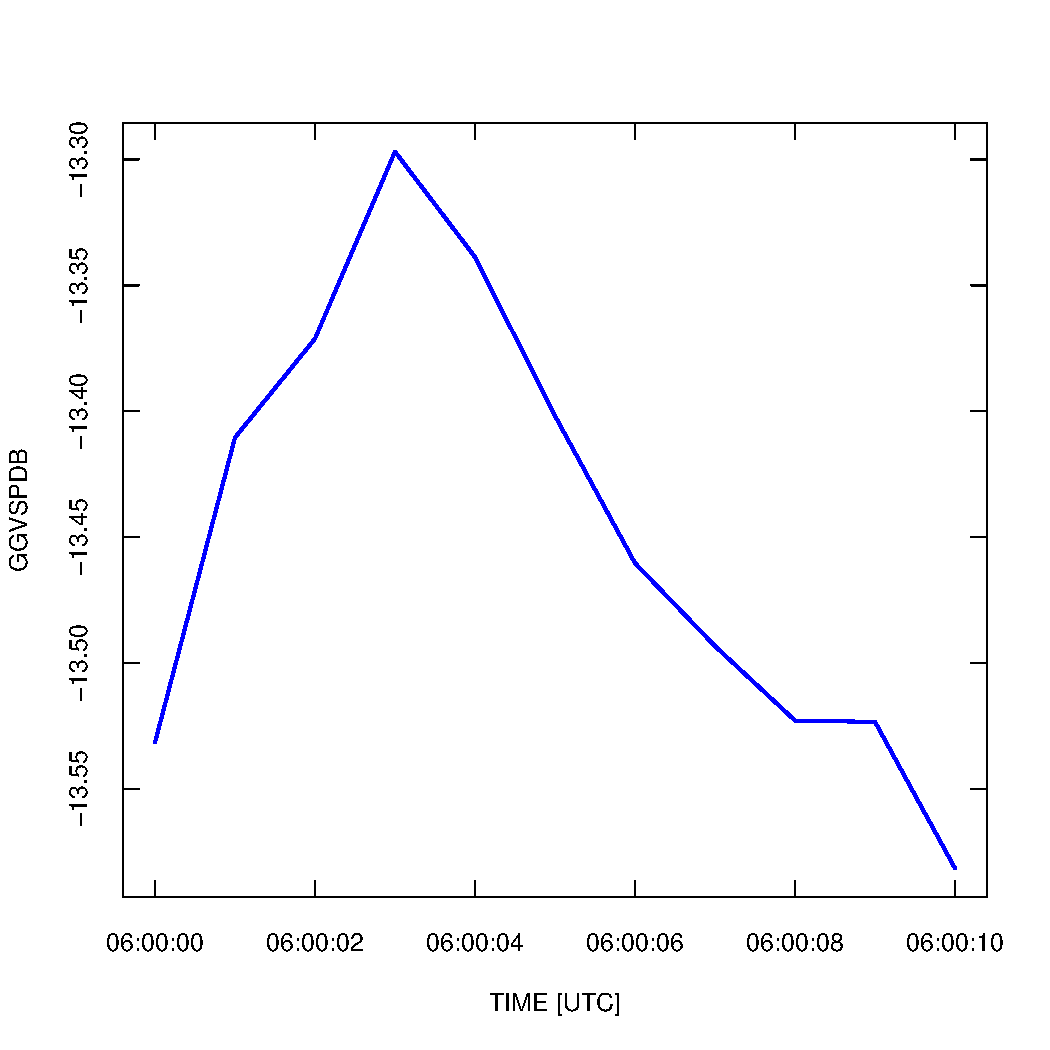
\includegraphics[width=\maxwidth]{figure/plot-GGVSPDB} 
\begin{kframe}\begin{verbatim}
## NULL
\end{verbatim}
\end{kframe}
\end{knitrout}

It is also useful to define special data.frames for constructing plots,
especially when using the more advanced plotting capabilities provided
by ggplot2. To see a simple scatterplot, you can use the following:

\begin{knitrout}
\definecolor{shadecolor}{rgb}{0.969, 0.969, 0.969}\color{fgcolor}\begin{kframe}
\begin{alltt}
\hlstd{D} \hlkwb{<-} \hlstd{Data[,} \hlkwd{c}\hlstd{(}\hlstr{"ATX"}\hlstd{,} \hlstr{"GGALT"}\hlstd{)]}
\hlkwd{plot}\hlstd{(D,} \hlkwc{pch}\hlstd{=}\hlnum{20}\hlstd{)}         \hlcom{# pch=20 plots small solid dots}
\end{alltt}
\end{kframe}
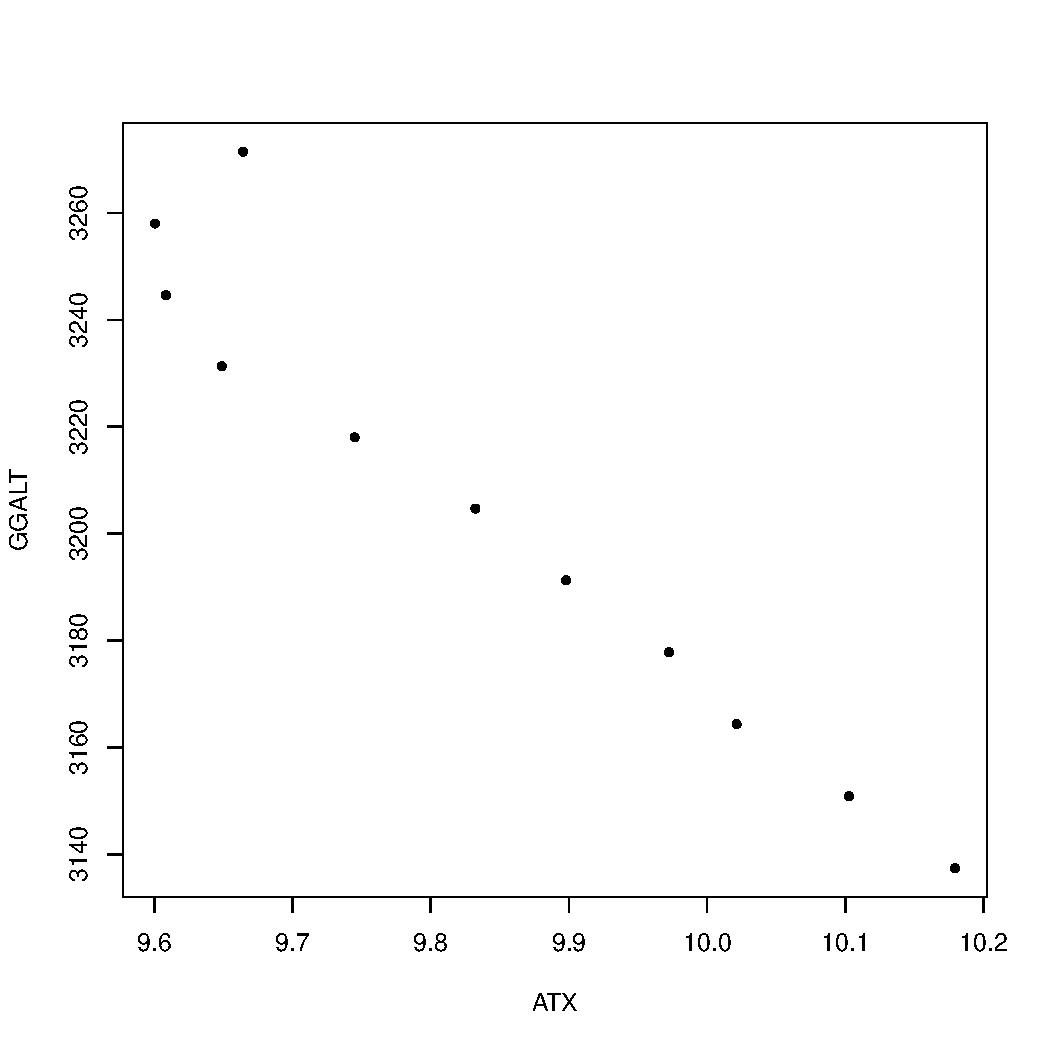
\includegraphics[width=\maxwidth]{figure/plot-df} 

\end{knitrout}

Exercise: See what happens if you instead include three variables
in the preceding plot.


\subsection*{Exporting to Excel}

and now create an Excel spreadsheet with the data:

\begin{knitrout}
\definecolor{shadecolor}{rgb}{0.969, 0.969, 0.969}\color{fgcolor}\begin{kframe}
\begin{alltt}
\hlkwd{require}\hlstd{(xlsx)}
\end{alltt}


{\ttfamily\noindent\itshape\color{messagecolor}{\#\# Loading required package: xlsx\\\#\# Loading required package: rJava\\\#\# Loading required package: xlsxjars}}\begin{alltt}
\hlkwd{write.xlsx} \hlstd{(Data,} \hlkwc{file}\hlstd{=}\hlstr{"Data.xlsx"}\hlstd{)}
\hlcom{#system("libreoffice Data.xlsx")}
\end{alltt}
\end{kframe}
\end{knitrout}

\begin{center}
\textsf{\textcolor{blue}{-- End of Memo --}}
\par\end{center}

Reproducibility:

\begin{tabular}{ll}
\textsf{\textsc{\textcolor{blue}{Project:}}} & RSessions\tabularnewline
\textsf{\textsc{\textcolor{blue}{Archive package:}}} & RSessionsDataFrame.zip\tabularnewline
\textsf{\textsc{\textcolor{blue}{Contains:}}} & attachment list below\tabularnewline
\textsf{\textsc{\textcolor{blue}{Program:}}} & /h/eol/cooperw/RStudio/RSessions/RSessionsDataFrame.Rnw\tabularnewline
\textsf{\textsc{\textcolor{blue}{Original Data:}}} & /scr/raf\_data/CONTRAST/CONTRASTrf08.nc\tabularnewline
\textsf{\textsc{\textcolor{blue}{Git:}}} & \tabularnewline
\end{tabular}

%\attach{attachment}

\attachm{ProgramFile\\Document.pdf\\SessionInfo\\RSessionsDataFrame.Rdata.gz}

\begin{knitrout}
\definecolor{shadecolor}{rgb}{0.969, 0.969, 0.969}\color{fgcolor}\begin{kframe}
\begin{alltt}
\hlkwd{sink} \hlstd{(}\hlkwc{file}\hlstd{=}\hlstr{"SessionInfo"}\hlstd{,} \hlkwc{type}\hlstd{=}\hlstr{"output"}\hlstd{)}
\hlkwd{print} \hlstd{(}\hlkwd{sessionInfo} \hlstd{())}
\end{alltt}
\begin{verbatim}
## R version 3.1.1 (2014-07-10)
## Platform: x86_64-redhat-linux-gnu (64-bit)
## 
## locale:
##  [1] LC_CTYPE=en_US.UTF-8          LC_NUMERIC=C                 
##  [3] LC_TIME=en_US.UTF-8           LC_COLLATE=en_US.UTF-8       
##  [5] LC_MONETARY=en_US.UTF-8       LC_MESSAGES=en_US.UTF-8      
##  [7] LC_PAPER=en_US.UTF-8          LC_NAME=en_US.UTF-8          
##  [9] LC_ADDRESS=en_US.UTF-8        LC_TELEPHONE=en_US.UTF-8     
## [11] LC_MEASUREMENT=en_US.UTF-8    LC_IDENTIFICATION=en_US.UTF-8
## 
## attached base packages:
## [1] grid      stats     graphics  grDevices utils     datasets  methods  
## [8] base     
## 
## other attached packages:
##  [1] xlsx_0.5.7            xlsxjars_0.6.1        rJava_0.9-6          
##  [4] Ranadu_0.0-2014-09-30 signal_0.7-4          reshape2_1.4         
##  [7] ggthemes_1.7.0        ggplot2_1.0.0         rPython_0.0-5        
## [10] RJSONIO_1.3-0         mapdata_2.2-3         mapproj_1.2-2        
## [13] maps_2.3-7            nleqslv_2.4           ncdf_1.6.7           
## [16] knitr_1.6            
## 
## loaded via a namespace (and not attached):
##  [1] colorspace_1.2-4 digest_0.6.4     evaluate_0.5.5   formatR_0.10    
##  [5] gtable_0.1.2     highr_0.3        MASS_7.3-33      munsell_0.4.2   
##  [9] plyr_1.8.1       proto_0.3-10     Rcpp_0.11.2      scales_0.2.4    
## [13] stringr_0.6.2    tools_3.1.1
\end{verbatim}
\begin{alltt}
\hlkwd{sink} \hlstd{()}
\hlkwd{system} \hlstd{(}\hlstr{"zip RSessionsDataFrame.zip RSessionsDataFrame.Rnw RSessionsDataFrame.pdf 
        SessionInfo RSessionsDataFrame.Rdata.gz"}\hlstd{)}
\end{alltt}
\end{kframe}
\end{knitrout}

%\cc{first attachment\\second\\3rd att}
\end{document}
